% Copyright (C) 2010,2011,2012 The ESPResSo project
% Copyright (C) 2002,2003,2004,2005,2006,2007,2008,2009,2010 
%   Max-Planck-Institute for Polymer Research, Theory Group
%  
% This file is part of ESPResSo.
%   
% ESPResSo is free software: you can redistribute it and/or modify it
% under the terms of the GNU General Public License as published by the
% Free Software Foundation, either version 3 of the License, or (at your
% option) any later version.
%  
% ESPResSo is distributed in the hope that it will be useful, but
% WITHOUT ANY WARRANTY; without even the implied warranty of
% MERCHANTABILITY or FITNESS FOR A PARTICULAR PURPOSE.  See the GNU
% General Public License for more details.
%  
% You should have received a copy of the GNU General Public License
% along with this program.  If not, see <http://www.gnu.org/licenses/>.
%
\documentclass[
a4paper,                        % paper size
11pt,                           % font size
twoside,                        % two sided
footsepline,                    % add a line to separate the footer
headsepline,                    % add a line to separate the header
headexclude,                    % header does not belong to the text
footexclude,                    % footer does not belong to the text
pagesize,                       % set the pagesize in a DVI document
]{scrartcl}

% Copyright (C) 2010,2011,2012 The ESPResSo project
% Copyright (C) 2002,2003,2004,2005,2006,2007,2008,2009,2010
%  Max-Planck-Institute for Polymer Research, Theory Group
%  
% This file is part of ESPResSo.
%   
% ESPResSo is free software: you can redistribute it and/or modify it
% under the terms of the GNU General Public License as published by the
% Free Software Foundation, either version 3 of the License, or (at your
% option) any later version.
%  
% ESPResSo is distributed in the hope that it will be useful, but
% WITHOUT ANY WARRANTY; without even the implied warranty of
% MERCHANTABILITY or FITNESS FOR A PARTICULAR PURPOSE.  See the GNU
% General Public License for more details.
%  
% You should have received a copy of the GNU General Public License
% along with this program.  If not, see <http://www.gnu.org/licenses/>.
%
\usepackage[draft]{varioref}    % defines \vref
\usepackage{hyperref}           % automatically creates links when
                                % using pdflatex, defines \url
\usepackage{ifpdf}              % defines \ifpdf
\usepackage{graphicx}           % handles graphics
\usepackage{color}              % use colors

\usepackage{amsmath}

\usepackage{verbatim}           % required for \verbatim and \endverbatim
\usepackage{fancyvrb}
\usepackage{calc}               % compute length
\usepackage{ifthen}             % provide ifthen
\usepackage{xspace}
\usepackage{units}
\usepackage[numbers]{natbib}

% For building the distribution docs, disable todo boxes.
%\usepackage[disable]{todonotes}
\usepackage{todonotes}

\newcommand{\es}{\mbox{\textsf{ESPResSo}}\xspace}
\newcommand{\ie}{\textit{i.e.}\xspace}
\newcommand{\eg}{\textit{e.g.}\xspace}
\newcommand{\etal}{\textit{et al.}\xspace}

\newcommand{\codebox}[1]%
{\texttt{#1}}

\DefineVerbatimEnvironment{code}{Verbatim}%
{commandchars=\\\{\}}
\makeatletter
\newenvironment{tclcode}
{%
  \addtolength{\linewidth}{-2em}% set the line length
  \@minipagetrue%%%DPC%%%
  \@tempswatrue%%%DPC%%%
  \hsize=\linewidth%
  \setbox0=\vbox\bgroup\verbatim
}{\endverbatim
  \unskip\setbox0=\lastbox%%%DPC%%%
  \egroup
  \par%
  \noindent\hspace{1em}%
  \codebox{\box0}%
  \par\noindent%
}
\makeatother

% \newcommand{\todo}[1]{
%   \marginpar{%
%     \setlength{\fboxrule}{1pt}
%     \fcolorbox{red}{yellow}{%
%       \parbox{\marginparwidth-2\fboxrule-2\fboxsep}{%
%         \bf\raggedright\scriptsize #1%
%       }%
%     }%
%   }%
% }

\makeatletter
\renewcommand{\minisec}[1]{\@afterindentfalse \vskip 1.5ex
  {\parindent \z@
    \raggedsection\normalfont\sffamily\itshape\nobreak#1\par\nobreak}%
  \@afterheading}
\makeatother

\newcommand{\esptitlehead}{
  \titlehead{
    \begin{center}
      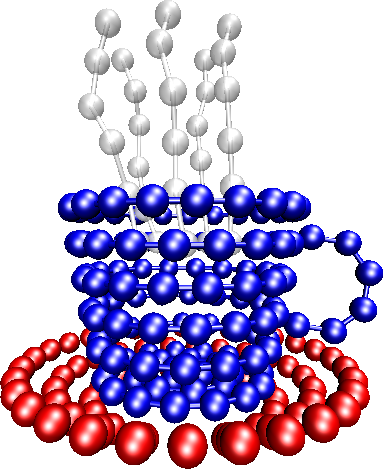
\includegraphics[width=5cm]{logo/transparentbg}
    \end{center}
  }
}


\begin{document}
\esptitlehead
\title{Tutorial 2: A simple charged system%
\ifdefined\esversion%
\thanks{For \es \esversion}%
\fi%
}

\maketitle
\tableofcontents

\section{Introduction}

This tutorial introduces some of the features of \es\ by constructing
step by step a simulation script for a simple salt crystal.  We cannot
give a full Tcl tutorial here; however, most of the constructs should
be self--explanatory. We also assume that the reader is familiar with
the basic concepts of a MD simulation here. The code pieces can be
copied step by step into a file, which then can be run using
\verb|Espresso <file>| from the \es source directory.

\section{Basic set up}

Our script starts with setting up the initial configuration.  Most
conveniently, one would like to specify the density and the number of
particles of the system as parameters:

\begin{tclcode}
  set n_part 200; set density 0.7
  set box_l [expr pow($n_part/$density,1./3.)]
\end{tclcode}

These variables do not change anything in the simulation engine, but
are just standard Tcl variables; they are used to increase the
readability and flexibility of the script. The box length is not a
parameter of this simulation; it is calculated from the number of
particles and the system density. This allows to change the parameters
later easily, e.~g.\ to simulate a bigger system.

The parameters of the simulation engine are modified by the
\verb|setmd| command. For example

\begin{tclcode}
  setmd box_l $box_l $box_l $box_l
  setmd periodic 1 1 1
\end{tclcode}
% make font-lock happy $

defines a cubic simulation box of size \verb|box_l|, and periodic
boundary conditions in all spatial dimensions. We now fill this
simulation box with particles

\begin{tclcode}
  set q 1; set type 0
  for {set i 0} { $i < $n_part } {incr i} {
    set posx [expr $box_l*[t_random]]
    set posy [expr $box_l*[t_random]]
    set posz [expr $box_l*[t_random]]
    set q [expr -$q]; set type [expr 1-$type]
    part $i pos $posx $posy $posz q $q type $type
  }
\end{tclcode}
% make font-lock happy $

This loop adds \verb|n_part| particles at random positions, one by
one.  In this construct, only two commands are not standard Tcl
commands: the random number generator \verb|t_random| and the
\verb|part| command, which is used to specify particle properties,
here the position, the charge \verb|q| and the type. In \es\ the
particle type is just an integer number which allows to group
particles; it does not imply any physical parameters. Here we use it
to tag the charges: positive charges have type 0, negative charges
have type 1.

Now we define the ensemble that we will be simulating. This is done
using the \verb|thermostat| command. We also set some integration
scheme parameters:

\begin{tclcode}
  setmd time_step 0.01; setmd skin 0.4
  set temp 1; set gamma 1
  thermostat langevin $temp $gamma
\end{tclcode}

This switches on the Langevin thermostat for the NVT ensemble, with
temperature \verb|temp| and friction \verb|gamma|. The skin depth
\verb|skin| is a parameter for the link--cell system which tunes its
performance, but cannot be discussed here.

Before we can really start the simulation, we have to specify the
interactions between our particles.  We use a simple, purely repulsive
Lennard-Jones interaction to model the hard core repulsion, and the
charges interact via the Coulomb potential:

\begin{tclcode}
  set sig 1.0; set cut [expr 1.12246*$sig]
  set eps 1.0; set shift [expr 0.25*$eps]
  inter 0 0 lennard-jones $eps $sig $cut $shift 0
  inter 1 0 lennard-jones $eps $sig $cut $shift 0
  inter 1 1 lennard-jones $eps $sig $cut $shift 0
  puts [inter coulomb 10.0 p3m tunev2 accuracy 1e-3 mesh 32]
\end{tclcode}

The first three \verb|inter| commands instruct \es\ to use the same
purely repulsive Lennard--Jones potential for the interaction between
all combinations of the two particle types 0 and 1; by using different
parameters for different combinations, one could simulate differently
sized particles.  The last line sets the Bjerrum length to the value
10, and then instructs \es\ to use P$^3$M for the Coulombic
interaction and to try to find suitable parameters for an rms force
error below $10^{-3}$, with a fixed mesh size of 32. The mesh is fixed
here to speed up the tuning; for a real simulation, one will also tune
this parameter. The \verb|puts| statement will show the parameters and
timings that the tuning found. Tuning takes some time; if you run many
simulations with similar parameters, you might want to save and reload
the P$^3$M parameters. You can obtain the P$^3$M parameters by
\verb|inter coulomb|:

\begin{tclcode}
  set p3m_params [inter coulomb]
\end{tclcode}

They are printed in a format suitable to feed them back to the
\verb|inter| command:

\begin{tclcode}
  eval inter $p3m_params
  eval inter $p3m_params
\end{tclcode}

\section{Running the simulation}

Now we can integrate the system:

\begin{tclcode}
  set integ_steps 200
  for {set i 0} { $i < 20 } { incr i} {
    set temp [expr [analyze energy kinetic]/((3/2.0)*$n_part)]
    puts "t=[setmd time] E=[analyze energy total], T=$temp"
    integrate $integ_steps
  }
\end{tclcode}

This code block is the primary simulation loop and runs
$20\times$\verb|integ_steps| MD steps. Every \verb|integ_steps| time
steps, the potential, electrostatic and kinetic energies are printed
out. The latter one is printed as temperature, by rescaling by the
number of degrees of freedom (3) multiplied by $1/2kT$. Note that
energies are measured in $kT$, so that only the factor $1/2$
remains. Also note that $3/2$ is written as $3/2.0$; otherwise Tcl
will perform an integer division, resulting in 1 instead of $1.5$.

Note, that in \es\ there are usually 3 translational degrees per
particle. However, if \verb|ROTATION| is compiled in, there are in
addition 3 rotational degrees of freedom, which also contribute to the
kinetic energy.  You can get this number in the following way
\footnote{Note: there also exists a predefined tcl function {\it
    degrees\_of\_freedom} which does the same.}:

\begin{tclcode}
  if { [regexp "ROTATION" [code_info]] } {
    set deg_free 6
  } {
    set deg_free 3
  }
\end{tclcode}

Then all you need to do is to replace the hardcoded 3 by \verb|$deg_free|.

However, if you run the simulation, it will still
crash: \es\ complains about particle coordinates being out of range.
The reason for this is simple: Due to the initial random setup, the
overlap energy is around a million kT, which we first have to remove
from the system. In \es, this is can be accelerated by capping the
forces, i.~e.\ modifying the Lennard--Jones force such that it is
constant below a certain distance. Before the integration loop, we
therefore insert this equilibration loop:

\begin{tclcode}
  for {set cap 20} {$cap < 200} {incr cap 20} {
    inter ljforcecap $cap
    integrate $integ_steps
  }
  inter ljforcecap 0
\end{tclcode}
% make font-lock happy $

This loop integrates the system with a force cap of initially 20 and
finally 200.  The last command switches the force cap off again. With
this equilibration, the simulation script runs fine. As a control
that the equilibration loop works correctly, you might want to add the
energy and force printing of the integration loop. You can then
observe how the temperature initially overshoots and then relaxes to
its target value by the action of the thermostat.

\section{Writing out data}

However, it takes some time to simulate the system, and one will
probably like to write out simulation data to configuration files, for
later analysis. For this purpose \es\ has commands to write simulation
data to a Tcl stream in an easily parsable form.  We add the following
lines at end of integration loop to write the configuration files
``config\_0'' through ``config\_19'':

\begin{tclcode}
  set f [open "config_$i" "w"]
  blockfile $f write tclvariable {box_l density}
  blockfile $f write variable box_l
  blockfile $f write particles {id pos type}
  close $f
\end{tclcode}
% make font-lock happy $

The created files ``config\_...'' are human--readable and look like

\begin{tclcode}
{tclvariable 
	{box_l 6.58633756008}
	{density 0.7}
}
{variable  {box_l 6.58633756008 6.58633756008 6.58633756008} }
{particles {id pos type} 
	{0 14.7658693713 29.5464807649 -17.5071728732 1}
	{1 26.702434508 -37.4986024417 114.617582522 0}
}
\end{tclcode}

As you can see, such a \emph{blockfile} consists of several Tcl lists,
which are called \emph{blocks}, and can store any data available from
the simulation. Reading a configuration is done by the following
simple script:

\begin{tclcode}
  set f [open $filename "r"]
  while { [blockfile $f read auto] != "eof" } {}
  close $f
\end{tclcode}
% make font-lock happy $

The \verb|blockfile read auto| commands will set the Tcl variables
\verb|box_l| and \verb|density| to the values specified in the file
when encountering the \verb|tclvariable| block, and set the box
dimensions for the simulation when encountering the \verb|variable|
block. The particle positions and types of all 216 particles are
restored when the \verb|particles| block is read. Note that it is
important to have the box dimensions set before reading the particles,
to avoid problems with the periodic boundary conditions.

\begin{figure}[tb]
  \centering
  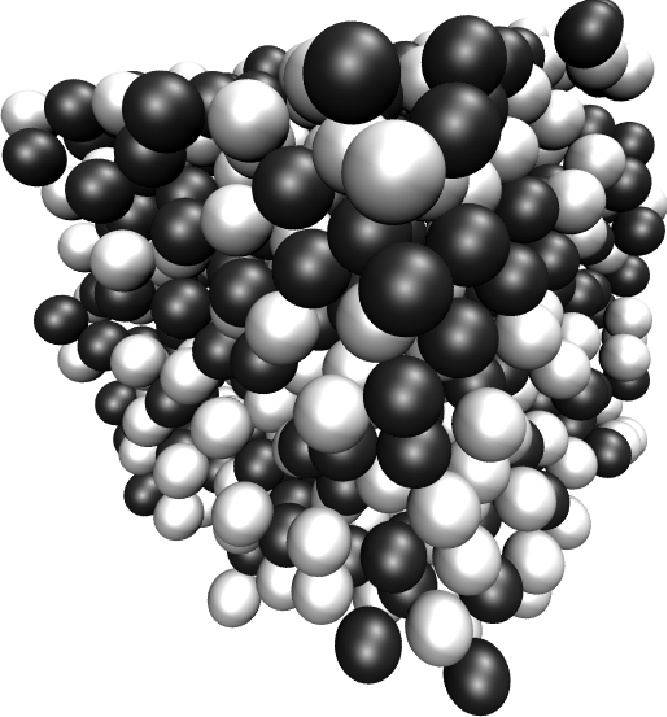
\includegraphics[width=0.4\textwidth]{figures/salt}
  \caption{VMD Snapshot of the salt system}
  \label{fig:snapshot}
\end{figure}

\section{Analysis}

With these configurations, we can now investigate the system. As an
example, we will create a second script which calculates the averaged
radial distribution functions $g_{++}(r)$ and $g_{+-}(r)$. The radial
distribution function for a the current configuration can be obtained
using the \verb|analyze| command:

\begin{tclcode}
  set rdf [analyze rdf 0 1 0.9 [expr $box_l/2] 100]
  set rlist ""
  set rdflist ""
  foreach value [lindex $rdf 1] {
    lappend rlist [lindex $value 0]
    lappend rdflist [lindex $value 1]
  }
\end{tclcode}

The shown \verb|analyze rdf| command returns the distribution function
of particles of type 1 around particles of type 0 (i.~e.\ of opposite
charges) for radii between $0.9$ and half the box length, subdivided
into $100$ bins.  Changing the first two parameters to either ``0 0''
or ``1 1'' allows to determine the distribution for equal charges. The
result is a list of $r$ and $g(r)$ pairs, which the following foreach
loop divides up onto two lists \verb|rlist| and \verb|rdflist|.

To average over a set of configurations, we put the two last code
snippets into a loop like this:

\begin{tclcode}
  set cnt 0
  for {set i 0} {$i < 100} {incr i} { lappend avg_rdf 0 }
  foreach filename [lrange $argv 1 end] {
    set f [open $filename "r"]
    while {[blockfile $f read auto] != "eof" } {}
    close $f
    set rdf [analyze rdf 0 1 0.9 [expr $box_l/2] 100]
    set rlist ""
    set rdflist ""
    foreach value [lindex $rdf 1] {
      lappend rlist [lindex $value 0]
      lappend rdflist [lindex $value 1]
    }
    set avg_rdf [vecadd $avg_rdf $rdflist]
    incr cnt
  }
  set avg_rdf [vecscale [expr 1.0/$cnt] $avg_rdf]
\end{tclcode}
% make font-lock happy $

Initially, the sum of all $g(r)$, which is stored in \verb|avg_rdf|,
is set to 0.  Then the loops over all configurations given by
\verb|argv|, calculates $g(r)$ for each configuration and adds up all
the $g(r)$ in \verb|avg_rdf|.  Finally, this sum is normalized by
dividing by the number of configurations. Note again the
``1.0/\$cnt''; also here, this
is necessary, since ``1/\$cnt'' is interpreted as an integer division,
which results in 0 for $\text{cnt}>1$.  \verb|argv| is a predefined
variable: it contains all the command line parameters. Therefore this
script should be called like
\begin{verbatim}
  Espresso <script> n_nodes [<config>...]
\end{verbatim}
where \verb|n_nodes| is the number of CPUs \es should be running
on. And because the first parameter is \verb|n_nodes|, we need to
strip it off, which we do by the \verb|lrange| list operation of Tcl.

\begin{figure}[tb]
  \centering
  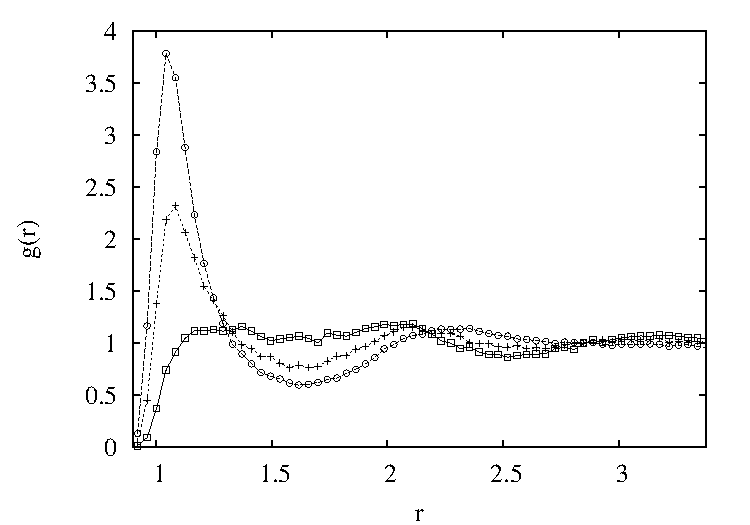
\includegraphics[width=0.7\textwidth]{figures/nacl-rdf}
  \caption{Radial distribution functions $g_{++}(r)$ between equal
    charges (rectangles) and $g_{+-}(r)$ for opposite charges
    (circles). The plus symbols denote $g(r)$ for an uncharged
    system.}
  \label{fig:rdf}
\end{figure}

The printing of the calculated radial distribution functions is
simple. Add to the end of the previous snippet the following lines:

\begin{tclcode}
  set plot [open "rdf.data" "w"]
  puts $plot "\# r rdf(r)"
  foreach r $rlist rdf $avg_rdf { puts $plot "$r $rdf" }
  close $plot
\end{tclcode}
%make font-lock happy: $

This instructs the Tcl interpreter to write the \verb|avg_rdf| to the
file \verb|rdf.data| in gnuplot--compatible format. Fig.~\ref{fig:rdf}
shows the resulting radial distribution functions, averaged over 100
configurations. In addition, the distribution for a neutral system is
given, which can be obtained from our simulation script by simply
removing the command \verb|inter coulomb ...| and therefore not
turning on P$^3$M.

The code example given before is still quite simple, and the reader is
encouraged to try to extend the example a little bit, e.~g. by using
differently sized particle, or changing the interactions. If something
does not work, \es\ will give comprehensive error messages, which
should make it easy to identify mistakes. For real simulations, the
simulation scripts can extend over thousands of lines of code and
contain automated adaption of parameters or online analysis, up to
automatic generation of data plots.  Parameters can be changed
arbitrarily during the simulation process, as needed for e.~g.\
simulated annealing. The possibility to perform non--standard
simulations without the need of modifications to the simulation core
was one of the main reasons why we decided to use a script language
for controlling the simulation core.

\section{Partially periodic boundary conditions}

\begin{figure}[t]
  \centering
  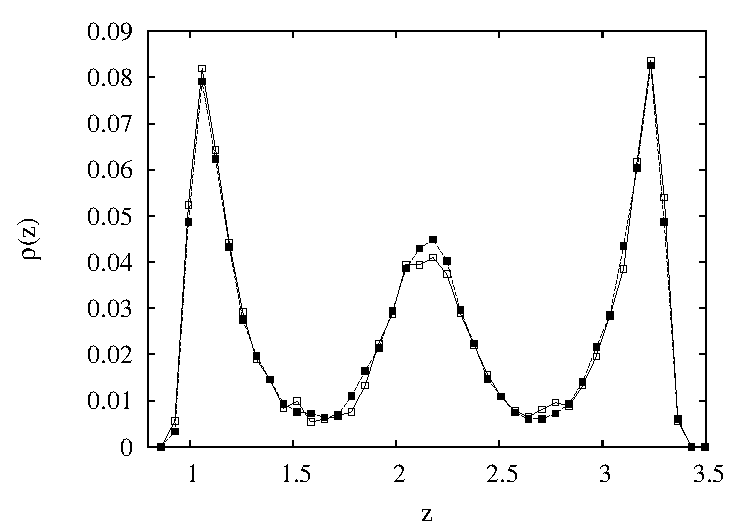
\includegraphics[width=0.7\textwidth]{figures/neutral-rho}
  \caption{Distribution of positive charges $\rho_+(z)$ (open squares)
    and of negative charges $\rho_-(z)$ (closed squares) under
    confinement along $z$.}
  \label{fig:neutralrho}
\end{figure}

One of the strengths of \es{} is the possibility to simulate charged
systems with partially periodic boundary conditions. As an example, we
will modify our script to simulate our simple salt in a slit pore. The
boundary conditions we define now as follows (note that you need the
\verb|PARTIAL_PERIODIC| feature):

\begin{tclcode}
  set box_lxy [expr sqrt(2)*$box_l]
  set box_lz  [expr 0.5*$box_l]
  setmd box_l $box_lxy $box_lxy [expr $box_lz + 1.0]
  setmd periodic 1 1 0
  constraint wall normal 0 0  1 dist 0 type 2
  constraint wall normal 0 0 -1 dist [expr -$box_lz - 1.0] type 2
\end{tclcode}

which replaces the previous code setting \verb|box_l| and
\verb|periodic|. The last two lines add two confining walls at the top
and the bottom of the simulation box. The wall is given by its normal
(pointing up and downwards here), and its distance from
$(0,0,0)$. Therefore this defines one wall passing at $z=0$, and a
second at $z=box_lz+1$. Finally, the type of the wall is used like a
particle type to define the interaction of the walls with the particles.

The addition of $1.0$ to the slit width is due to the fact that we will
use a Lennard-Jones potential to model the wall; this means that
particles of diameter $1.0$ cannot come closer than $1.0$ to the wall. In a
way, the wall itself therefore has a thickness of $0.5$. To compensate
for this, we simply make the box bigger by 1.

We also need to choose the initial positions of our particles to match
the new box dimensions. The particles are generated as before, but we
draw the random position now as follows:

\begin{tclcode}
  set posx [expr $box_lxy*[t_random]]
  set posy [expr $box_lxy*[t_random]]
  set posz [expr ($box_lz-1.0)*[t_random] + 1.0]
\end{tclcode}
%make font-lock happy: $

When defining the interactions, we now also need to add the
interactions between the particles and the walls, which is the same as
between the particles:

\begin{tclcode}
  inter 0 2 lennard-jones $eps $sig $cut $shift 0
  inter 1 2 lennard-jones $eps $sig $cut $shift 0
\end{tclcode}

For the electrostatic part, we also need to choose another algorithm,
as P$^3$M can only handle fully periodic boundary conditions. We
choose the MMM2D method:

\begin{tclcode}
  cellsystem layered 3
  inter coulomb 1.0 mmm2d 1e-4  
\end{tclcode}

which replaces the \verb|inter coulomb 10.0 p3m ...| code. Note the
decreased Bjerrum length --- the confined system would take too long for
a tutorial to equilibrate with Bjerrum length 10.0. Still,
equilibrating the system is now more difficult. First, we cannot
simply ramp up all Lennard-Jones interactions anymore; otherwise,
particles will penetrate the walls and break the confinement. Second,
we need to ramp up the electrostatic interaction more carefully
now. The following code gradually increases the Bjerrum length to the
target value of 1.0, and caps only the Lennard-Jones interactions
between the particles. The latter can be done by switching on
individual force capping, and setting a force cap radius for the
particle-particle interactions:

\begin{tclcode}
inter ljforcecap individual
for {set i 1} {$i < 10} {incr i} {
    set rad [expr 1.0 - 0.5*$i/10.0]
    set lb [expr 1.0 * $i / 10.0]
    inter 0 0 lennard-jones $eps $sig $cut $shift 0 $rad
    inter 1 0 lennard-jones $eps $sig $cut $shift 0 $rad
    inter 1 1 lennard-jones $eps $sig $cut $shift 0 $rad
    inter coulomb $lb mmm2d 1e-4
    integrate $integ_steps
}
inter ljforcecap 0
inter coulomb 1.0 mmm2d 1e-4  
\end{tclcode}
%make font-lock happy: $

Finally, when writing out, we should update the set of
Tcl-variables to represent the asymmetric box, and write out
\verb|box_lxy| and \verb|box_lz| instead of just \verb|box_l|.

\subsection*{Analysis}

For a such a strongly confined system, the radially averaged
distribution function is inappropriate. Instead, it would be more
interesting to study the distribution of the particles along the slit
width. \es{}  does not provide such a function, however, we can easily
write one using the \verb|bin| command, which simply allows to bin a
set of values given as a Tcl-list. Therefore, we first create the list
of z-coordinates, and then bin them:

\begin{tclcode}
  set data ""
  for {set p 0} {$p <= [setmd max_part]} {incr p} {
    lappend data [lindex [part $p pr pos] 2]
  }
  set rho [bin -linbins 0.5 [expr $box_lz + 0.5] $bins $data]
\end{tclcode}
%make font-lock happy: $

Here, \verb|bins| is a variable that you should set to the required
number of bins (20 should be fine). Otherwise, this code can replace
the analyze rdf command. The \verb|bin| command also allows to obtain
the coordinates of the bins:

\begin{tclcode}
  bin -linbins 0.5 [expr $box_lz + 0.5] $bins -binctrwdth
\end{tclcode}

will return a list of the centers and widths of the bins, which can be
used in analogy to \verb|rlist| in the previous analysis code. Of
course, it would be interesting to study the distribution of positive
and negative charges separately; for this, you need to duplicate the
averaging code, and use two data sets to append the z-coordinates to,
depending on the particle type:

\begin{tclcode}
  if {[part $p pr type] == 0} {
    lappend data0 [lindex [part $p pr pos] 2]
  } {
    lappend data1 [lindex [part $p pr pos] 2]
  }
\end{tclcode}
%make font-lock happy: $

The resulting distribution of charges is shown in
Fig.~\ref{fig:neutralrho}, showing a layering effect of the
confinement on the charge distributions.

\begin{figure}[t]
  \centering
  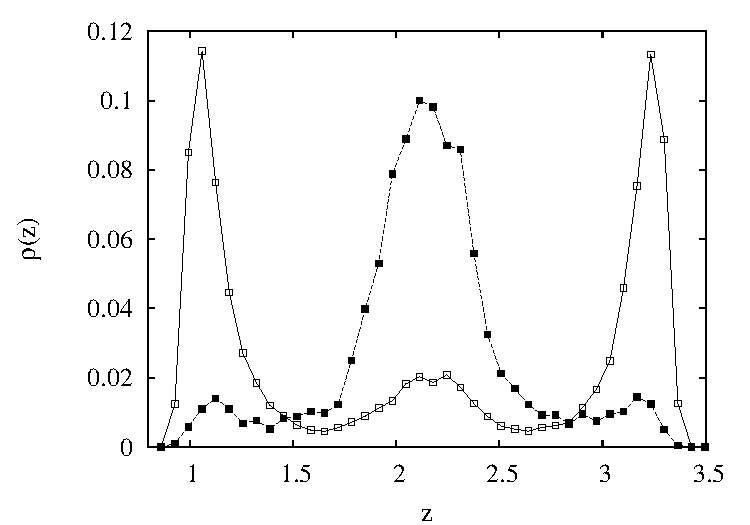
\includegraphics[width=0.7\textwidth]{figures/nonneutral-rho}
  \caption{Distribution of positive charges $\rho_+(z)$ (open squares)
    and of negative charges $\rho_-(z)$ (open squares) under
    confinement along $z$. The two confining walls are negatively
    charged, pushing away the negative charges.}
  \label{fig:nonneutralrho}
\end{figure}

\subsection*{Charging the walls}

So far, the distributions of particles of type 0 and 1 are more or
less the same, as one would expect. However, we can change this by
introducing charged walls. That is done using the
\verb|constrain plate| command:

\begin{tclcode}
  set sigma [expr -0.25*$n_part/($box_lxy*$box_lxy)]
  constraint plate height 0 sigma $sigma
  constraint plate height [expr $box_lz + 1.0] sigma $sigma
\end{tclcode}

This adds two plates at the bottom and top of the simulation box. The
charged walls (the condensator \emph{plates}) are necessarily
perpendicular to the z-axis, since for all electrostatics methods for
2d-periodic systems, the z-axis is the non-periodic one. Note that
this adds two walls with a total charge of \verb|n_part|/2, which
would make the overall system charged. To maintain charge neutrality,
we simply choose only half of the charges (i.e. 100) with altering
charge as before, while the rest we simply choose all with positive
charge. For this system, you should obtain distributions as shown in
Fig.~\ref{fig:nonneutralrho}. The distribution of charges differs
strongly between the two types of charges; while the positive charges
layer at the walls, the negative charges accumulate in the center of
the system.

\end{document}
